\chapter{Data acquisition software}

\epigraph{Before software can be reusable \\it first has to be usable.}{Ralph Johnson}

Data acquisition is a critical component of all particle physics experiments across all stages of technological readiness, from the very beginning of hardware testing in tabletop experiments to full-scale international experiments like the Large Hadron Collider. 

In the modern era of particle physics, the interplay of hardware and software at minscule timescales drives everything, and almost all results are highly dependent upon the speed and efficiency of the electronics and computer systems that extract data from the detectors. A massive quantity of work goes into creating, testing and optimising the systems that will acquire, process, sort and transport data before it is ever seen by the physicist running the experiment.

Of particular interest is the data acquisition software during the development phase where individual detector subcomponents are undergoing prototyping and testing. These development and iteration cycles are tied closely to testbeam facillities such as the Super Proton Synchrotron (SPS) at CERN and the DESY II synchrotron at DESY. At this point in the development cycle, the detectors are beginning to take shape and this is where data acquisition (or DAQ) becomes an important consideration. 

In addition to this, the data acquisition solutions used during the testbeam phase of detector development is likely to inform the final data acquisition solution, either directly by evolving into the final software, or indirectly by identifying and evaluating the particular features or challenges of the subdetector components that the software must take into account or accommodate.

During this stage, each individual detector component -- such as a vertex tracker or hadronic calorimeter -- will be developed by small teams, and the natural tendency is for each of these groups to set their own standards and develop their own tools, prioritising the features that are important to their specific case. However, in the past this approach has generated a variety of \textit{ad hoc} solutions for testbeam software, many of which cannot be applied outside of their original scope. The also results in wasted effort and time, as different teams implement the same solutions anew for each subdetector.

One of the aims of the AIDA-2020 project is to improve this situation by developing generic and reusable software tools for testbeams and particle physics experiments.

\subsubsection{The AIDA-2020 project}
The AIDA-2020 project is an EU-funded research programme for developing infrastructure and technologies for particle physics detector development and testing, comprising 24 member countries and lead by CERN.

The overarching goal of the project is to develop common infrastructures and tools for physics testbeams, and software is one such important tool. By creating a suite of tools that are designed with a variety of uses in mind, the amount of effort and development time necessary to plan and implement data acquisition and monitoring setups can be significantly reduced or eliminated, speeding up the planning and deployement of physics testbeams. This allows more science to be done faster. The two tools within AIDA-2020 that facillitate this are EUDAQ and DQM4HEP, discussed in more detail below.

\section{EUDAQ}
[...]

\section{DQM4HEP}
DQM4HEP is an online monitoring and data quality monitoring tool developed for physics testbeams for high-energy and particle physics. It is designed to be able to fulfil the requirements of monitoring for physics testbeams in a generic way. The structure of the program allows for independent components of the framework to be used, not used, or exchanged, by isolating each function of the program into specific and independent processes. The components that are specific to particular users -- the analysis and standalone modules -- are written in standard C++ code, meaning they are capable of performing any data unpacking, processing or analysis that is necessary. The framework then handles packaging this information in a useful way and networking to transmit it to where it is needed, meaning that the user does not have to worry about the mechanics of data storage, serialisation or transmission. It also means that the framework does not need special rules for handling particular datatypes, allowing it to handle \emph{anything} that can be packed into, decoded from, and accessed by normal C++ methods. This results in a framework that is able to deal with any kind of data, including user-defined data types, making it more flexible, portable and easily reusable.

\subsection{Prerequisites and dependencies}

DQM4HEP is a C++ application, written in the C++11 standard, that can run on Windows, OSX, or any Linux distribution [?]. 

Since DQM4HEP is designed to be modular, there are two tiers of requirements. Core requirements, that are necessary for the compilation and operation of the core program, and secondary requirements, which are necessary for certain modules or plugins that are optional.

[...]

\subsection{Programming paradigms and structure}
[...]

\begin{figure}[h]
	\centering
	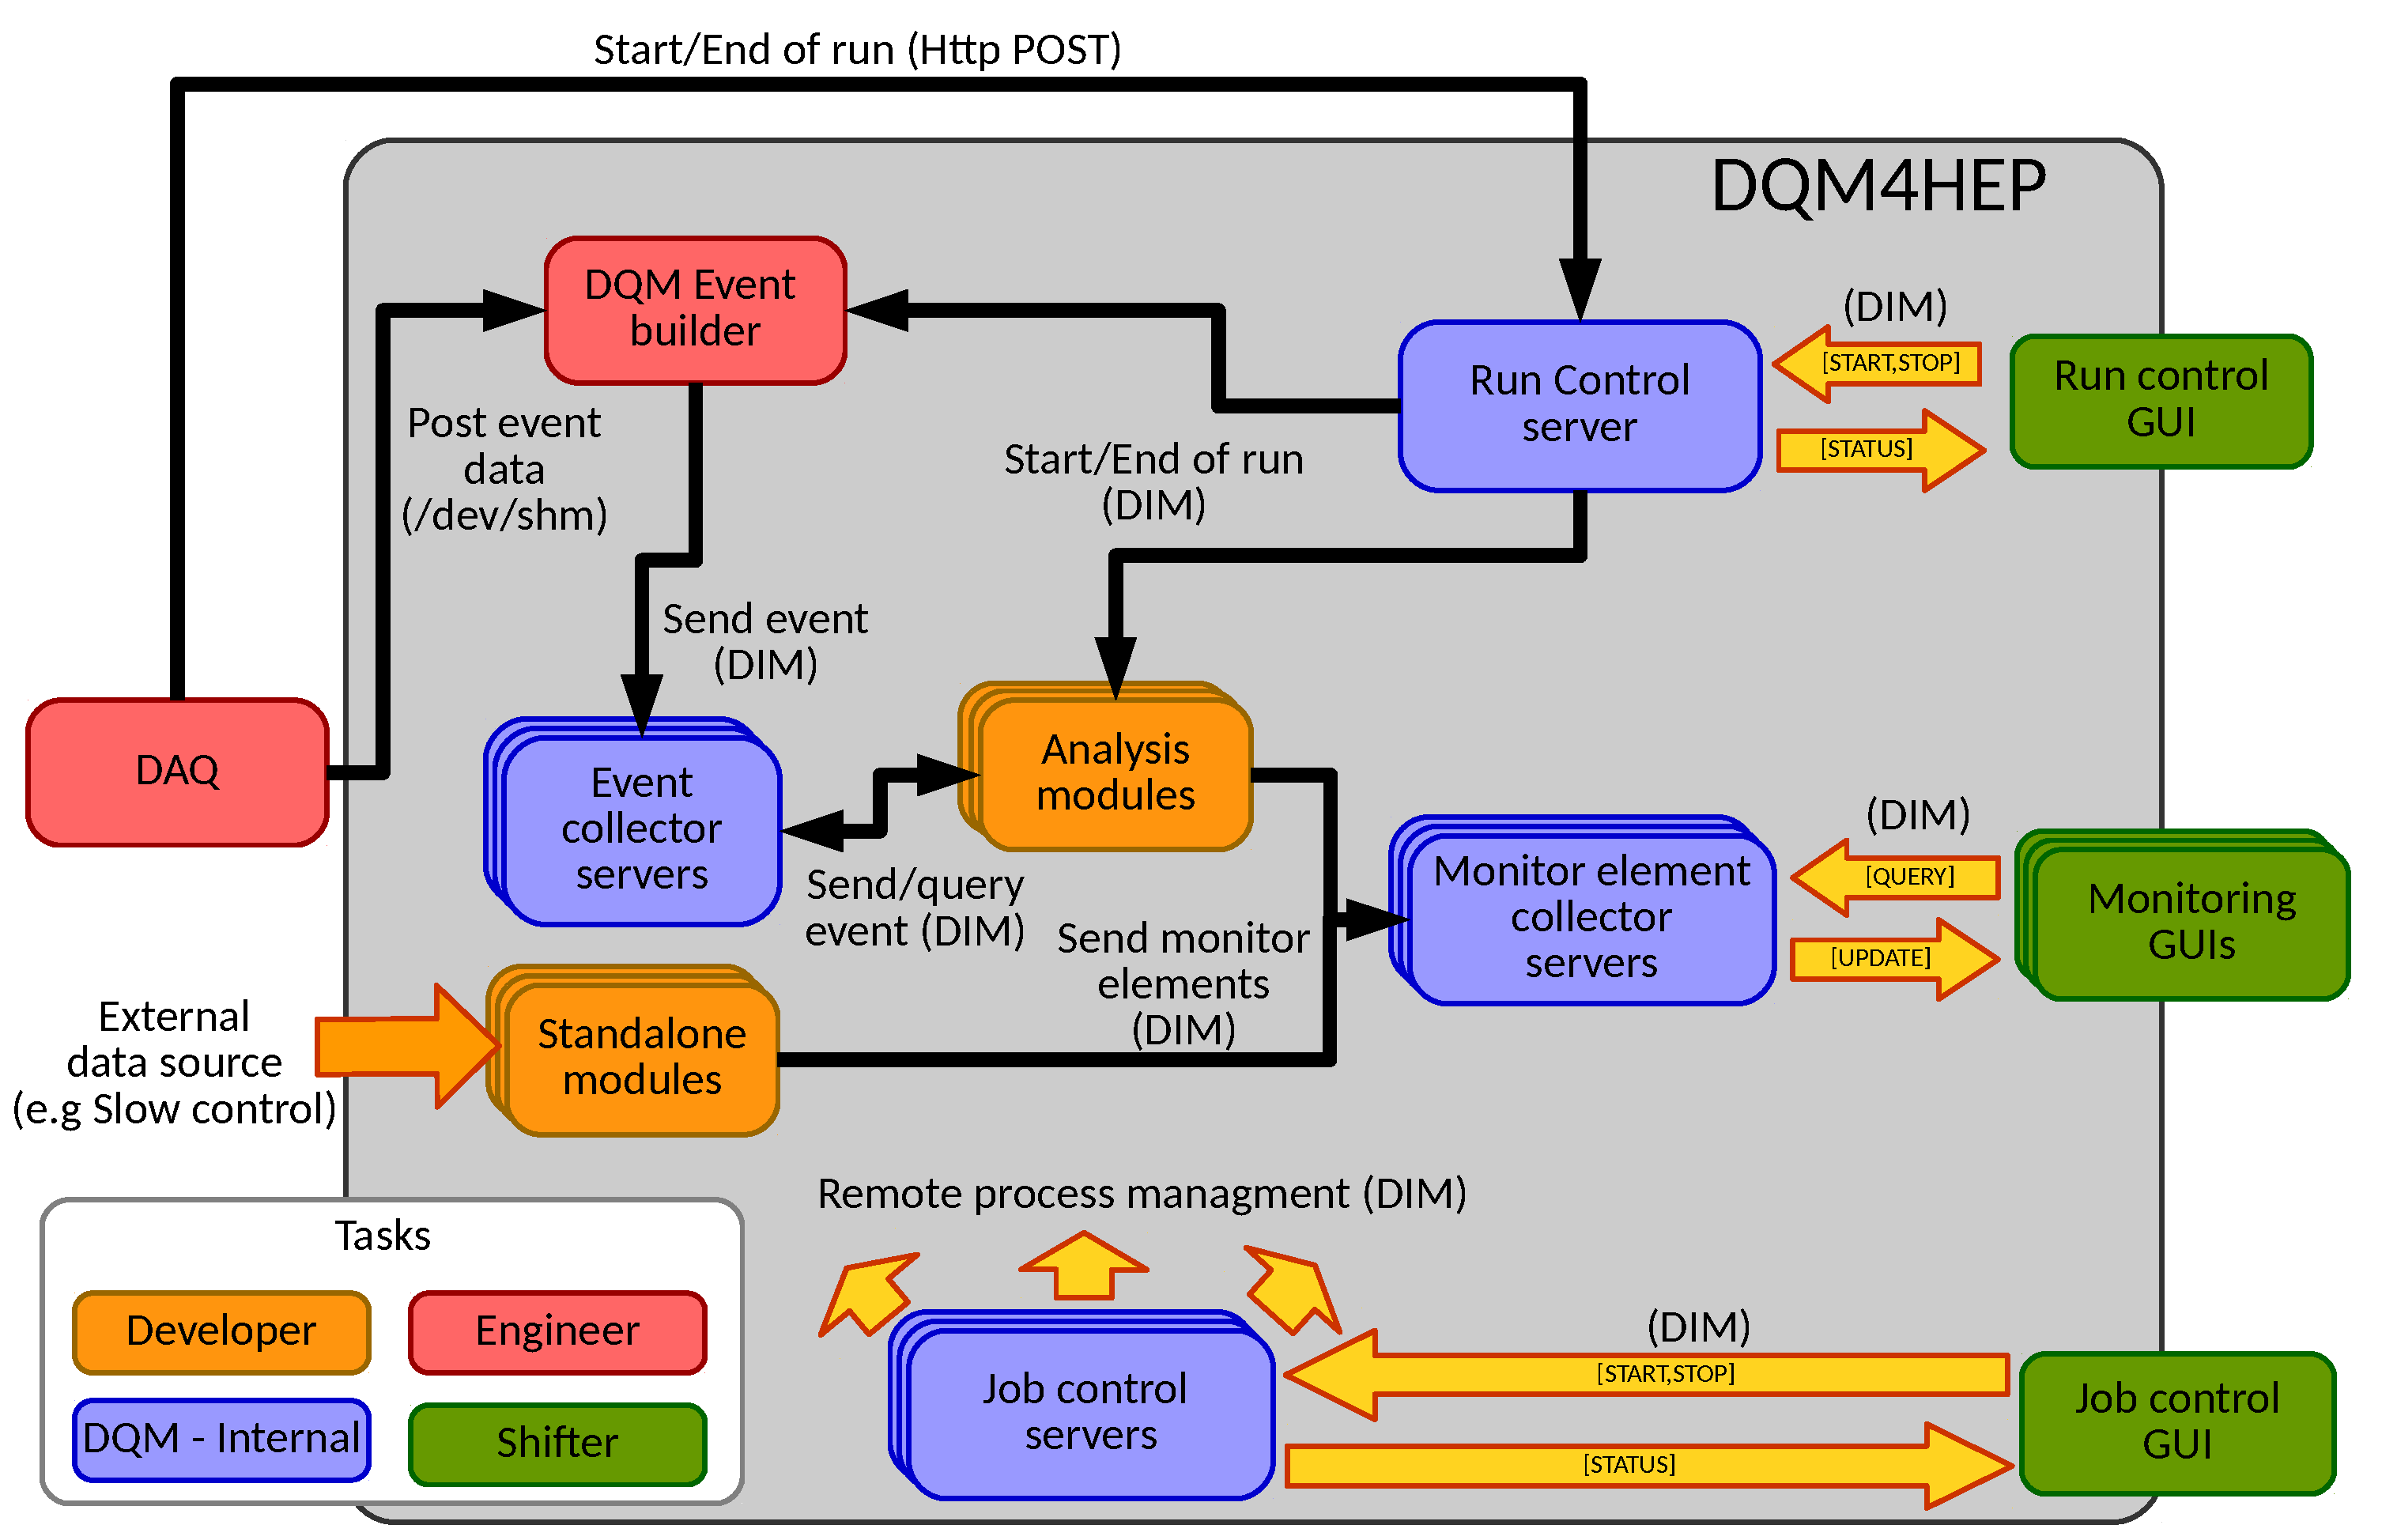
\includegraphics[width=0.95\textwidth]{../Pictures/GlobalArchitectureDiagram.pdf}
	\caption{The global online architecture of DQM4HEP.}
	\label{figure:daq/dqm4hep/architecture}
\end{figure}

\subsection{Visualisation and graphical user interface}
[...]

\subsection{Data quality testing}
One of the important areas of DQM4HEP that was not yet completed was data quality monitoring, which is an array of tests or programs that assess the data being taken in real time to allow testbeam operators and shifters without detailed knowledge of the hardware, software, or physics to determine whether the device under test is performing as intended, and to quickly identify and address any errors or inconsistencies. Data quality monitoring (DQM) uses a variety of methods for measuring the `quality' or `goodness' of data, mainly relying upon statistical or comparative methods.

DQM4HEP did not have any infrastructure to support data quality tests, but this was added during the core refactoring for the release version [?]. Once this was in place, a variety of data quality tests were developed and implemented, ranging from basic tests, such as comparing the mean of a data sample against predefined values of mean and standard deviation, to more complex tests, such as the Kolmogorov-Smirnov test, which is a comparison between a sample and a reference histogram.

[Illustrative pictures would go here; one of a pair of histograms demonstrating the quality of data with a mean/stddev test, and the other demonstrating a reference histogram, then by the side of it a picture of a sample histogram compared to the reference, maybe colour-highlighted?]

[...]

\section{Adaptation to other detectors}
[...]

\section{Integration with EUDAQ}
[...]

\section{Documentation and user guide}
[...]
